% status: 100
% chapter: Apache Spark

\title{Apache Spark}


\author{Saurabh Swaroop}
 \affiliation{%
  \institution{Indiana University Bloomington}
  \city{Bloomington} 
  \state{Indiana} 
  \postcode{47408}
  }
\email{sswaroop@iu.edu}

\author{Gregor von Laszewski}
\affiliation{%
  \institution{Indiana University}
  \streetaddress{Smith Research Center}
  \city{Bloomington} 
  \state{IN} 
  \postcode{47408}
  \country{USA}}
\email{laszewski@gmail.com}


% The default list of authors is too long for headers}
\renewcommand{\shortauthors}{G. v. Laszewski}


\begin{abstract}

Spark is an Apache open source project originally developed in AMP Lab at UC
Berkeley. It is a cluster computing framework which is built on top of Hadoop
distributed file system HDFS for data analysis and processing. Unlike Hadoop,
Spark does not use Map-reduce engine to read and write to hard disk.
It is based on, in memory computation process which increases its speed over
100X as compared to Hadoop. Spark has very tight integration of components and
also, inexpensive.

\end{abstract}

\keywords{hid-sp18--522,Big Data,Distributed Frameowrk,Machine Learning Computing
          Feature Extraction, Parallel Processing}


\maketitle


\section{Introduction}

The amount of data consumed and generated by enterprise are huge in current world.
Such large volume of data has created a necessity for the companies to make the
best use of the diversity and hidden information associated with them. Not only
these informations improvise the productivity but enables enterprises to identify
new opportunities.With the advent of big data, more enterprises are incorporating
data analytics when building strategic applications and making decisions. Data
processing and its effective analysis plays a very important role in functioning
and getting ahead of the competition for almost every enterprise now a days.


Enterprises need to have a standard process and infrastructure to perform data
analysis which involves several stages like Data Collection, Data Cleaning,
Data Storage, Data Processing, Data Analysis. On top of these stages lies the
models on which enterprise map their business to get ahead of their peers.


Apache Spark is cluster computing framework which is used for data processing
and analysis over large scale with great processing rate. It is one of most
popular framework being used for data analytics and processing due to its
several advantages like speed, easiness and cost effectiveness.


\section{Spark Overview}

In memory cluster computing framework allows applications to load data into a
cluster memory. This process enables multiple recursive queries without
performance overhead. It allows both batch and real-time data analytic and
processing pay loads. Spark can be installed over cluseter managers like
Hadoop Yarn, Apache Mesos or standalone Spark cluster. Spark can process data
from variety of sources like HDFS, Amazon S3, Cassandra etc. It supports file
formats like text files,avro,parquet and other hadoop input formats.

Spark has several applications as below:

\begin{itemize}
   \item Batch Applications 
   \item SQL
   \item Machine Learning
   \item Streaming Data Processing
   \item Graphical Data Processing  
\end{itemize}

Spark is available for Linux, OSX and Windows. It integrates well with several
languages like Java, Scala and Python. It provides an optimized engine that
supports general execution graphs. It also supports a rich set of higher-level
tools including Spark SQL for SQL and structured data processing, MLlib for
machine learning, GraphX for graph processing, and Spark Streaming.


\begin{figure}[!ht]
  \centering\includegraphics[width=\columnwidth]{images/sparkfeatures.png}
  \caption{Features
  of Spark~\cite{hid-sp18-522-sparkfeatures-image} }\label{f:fig1}
\end{figure}


\section{Spark Engine}

{\bf Spark Core} is the base engine for large-scale parallel and distributed data processing.
It contains basic spark functionalities like Task Scheduling, Memory management, Fault
Recovery and Interacting with storage systems. It also provides an API that defines RDD's


Spark is built around  RDD (Resilient Distributed Dataset). Resilient Distributed datasets
is basically a distributed collection of immutable data which is fault tolerant and
has ability to use many datasets. It supports parallel and partitioned operation. With
the release of Spark 2.0, RDD's are being replaced with Dataframes but Files are still
being distributed as RDD's. RDDs support two types of operations. First one is
Transformation which includes operations like FlatMap, Filter, Join etc. Second
operation is Action where the actual magic happens. Action comprises of functions
like Reduce, Count, collect etc.


{\bf Transformations} in Spark are lazy, which basically means that they don't perform any
function on the cluster until action is called. Transformation gets the access to dataset and
learns the future action to be performed on them. The transformations are executed  when an
action is called, and the result is returned to the driver program. During Transformation Spark
creates a DAG (Directed Acyclic graph). DAG has a map which contains execution of RDD
transformations. Transformation can be of two types:

\begin{itemize}
   \item Narrow Transformation: Map, Filter, Sample, Union
   \item Wide Transformation: Intersection, Join, Reduce by key
\end{itemize}

{\bf Action} actually triggers execution on cluster. When action is called on Spark RDD then Spark
submits graph to DAG scheduler. Operators are divided into stages of task in DAG scheduler.
The stages are passed on Task Scheduler which are launched through cluster manager.

\section{Spark Architecture}

{\bf Spark core has three major components:}

\begin{itemize}
   \item Main driver program also known as Spark Context or Spark Session 
   \item Cluster Manager
   \item Executer
\end{itemize}

\subsection{Spark Driver}

{\bf Spark driver} runs over master system. Whenever a spark application is submitted, then main function
is run by the master. Spark context is created inside driver and other components like task
scheduler and DAG scheduler reside within it. Driver runs over master node and negotiates with
cluster manager to schedule tasks.

\subsection{Cluster Manager}

They are pluggable components which means that it can be used with Yarn, Apache Mesos or standalone
spark cluster. Its primary function is to allocate and de-allocate resources.


\subsection{Executer}

{\bf Excecuters} run on slave systems.They are distributed over different systems within cluster. Single
executer may perform multiple tasks. It reads, processes and writes data related to the allocated
task. It may write data into memory, disk and cache.

\section{Spark Libraries}

Spark has other components tightened with it in form of libraries which are very useful in
multiple data analysis, machine learning and data processing applications. These libraries currently
include GraphX, MLlib, SparkSQL and Spark Streaming. Spark core and these bundled libraries
together form Spark architecture

\begin{figure}[!ht]
  \centering\includegraphics[width=\columnwidth]{images/Sparkarchitecture.png} \caption{Spark
  architecture}\label{f:fig2}
\end{figure}

\subsection{SparkSQL}

{\bf SparkSQL} module is the library to process structured data in the form of MySQL, Avro,Parquet
etc. SparkSQL gets started with SparkSession and it manipulates data in two ways. One through Dataframe
or dataset api's and other through sql queries. Dataframes are distributed collection of data
organized into named columns. Pandas library of python or R language provide dataframes.

Dataframes can be created in two ways:

\begin{itemize}
   \item From an existing RDD either with schema inference or with an explicit schema
   \item Reading in a specific data source from file
\end{itemize}

SparkSQL allows to create dataframe from variety of sources like Json, avro,ORC, Hive, Hbase,
cassandra, couchbase etc. It also has two backend components. Catalyst component is  query optimizer
which optimizes the code. Another component is Tungsten which is off heap serializer.
 

\begin{figure}[!ht]
  \centering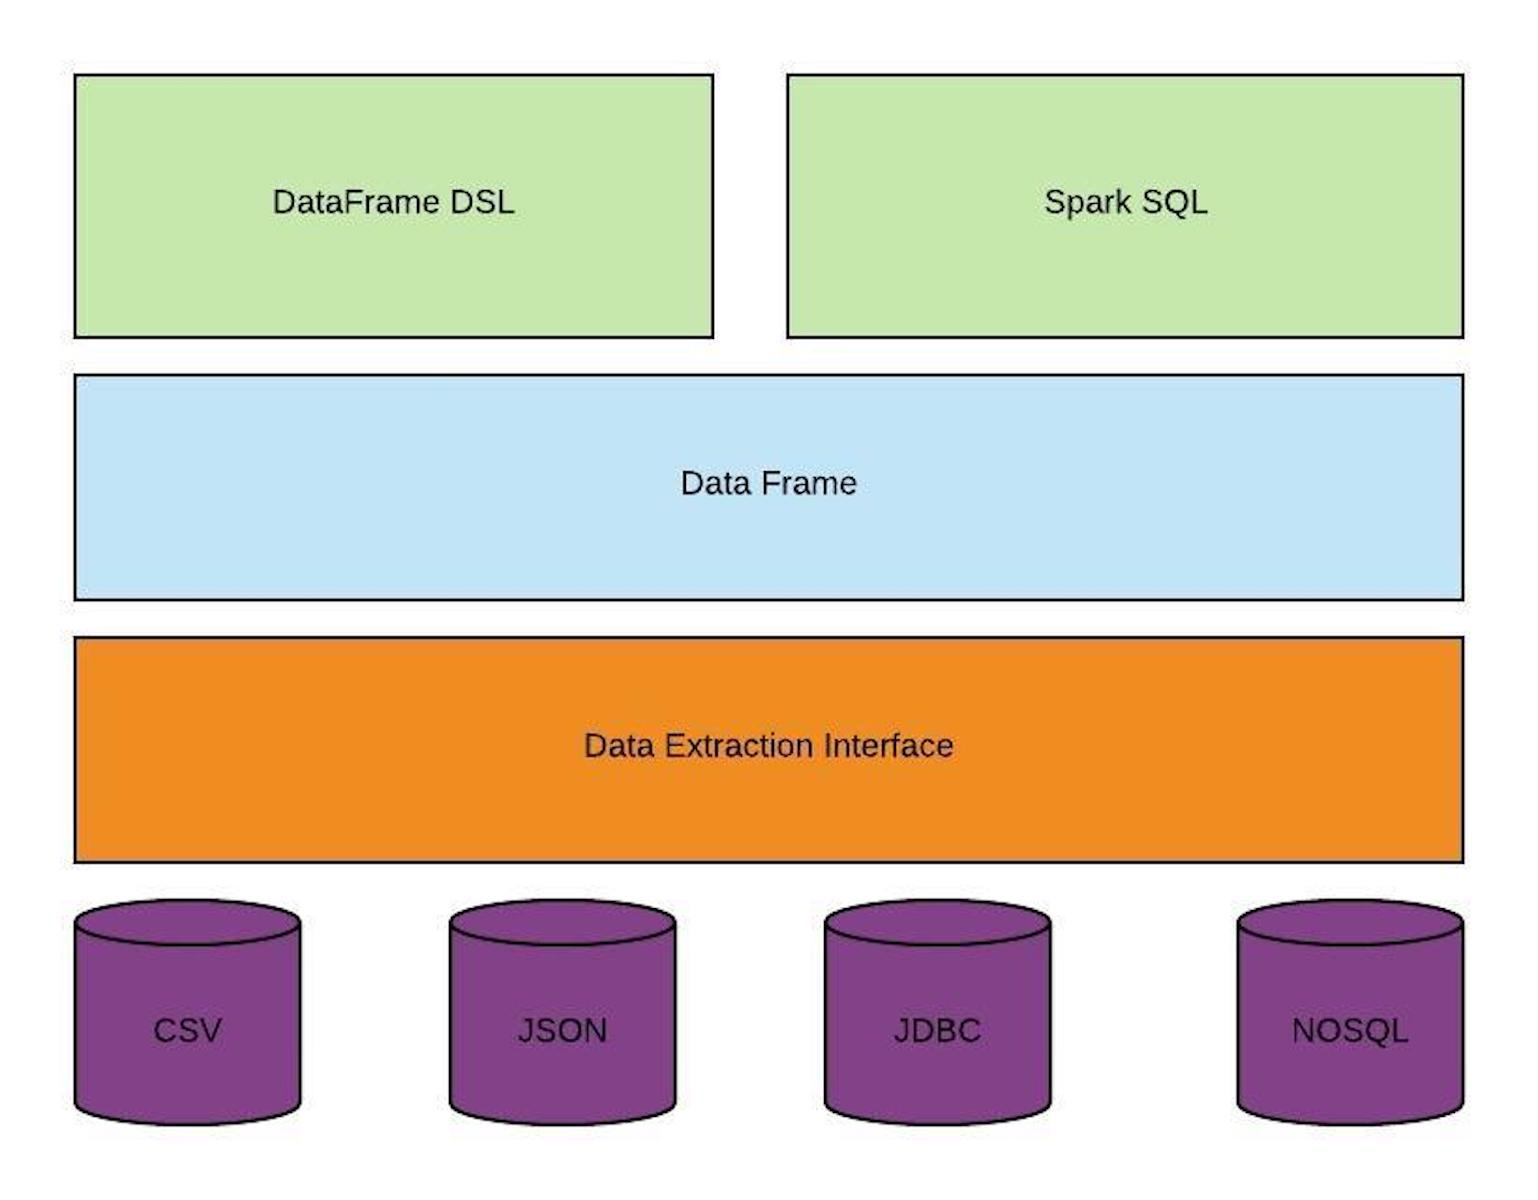
\includegraphics[width=\columnwidth]{images/sparksql.jpeg} \caption{Spark
  SQL}\label{f:fig3}
\end{figure}


\subsection{Spark Streaming}

The most powerful feature of spark is its high speed processing capability for massive datasets. One
of the desire in data processing is to process it in real time in contrary to batch or periodic
processing. Spark Streaming provides the capability to analyze and process data in real time instead
of huge batch jobs. One of the use case is to analyze streams of web server data and run some
business logic around them. Spark streaming is also the technology for IoT. The highlevel flow of
spark streaming starts from receiving data streams and distributing it over RDD's. This process of 
receiving the data stream and splitting them into small chunks or RDD's is called De-Streaming.
Data are then processed, transformed and sent to databases or other systems. Processing of chunks
of data over different RDD's can happen in parallel on different worker nodes. This basically
distributes massive data into smaller groups over clusters and hence gives a huge performance boost.


\begin{figure}[!ht]
  \centering\includegraphics[width=\columnwidth]{images/sparkstream.png} \caption{Spark
  SQL~\cite{hid-sp18-522-sparkstream-image} }\label{f:fig4}
\end{figure}

\subsection{MLlib}

{\bf Spark MLlib} is a party of Spark ecosystem which comes bundles with Machine Learning algorithms
and utilities which can run in parallel on Spark clusters. It has few new data types like Vector,
Labeled point. Vectors can be local or distributed over multiple RDD's. MLlib allows to invoke
multiple algorithms and models on distributed datasets and on different nodes within the cluster.

Spark MLlib has two components as below:

spark.mllib: It is built on top of Spark abstraction unit RDD and has several utilities like
Linear Algebra and statistics used in modelling. It comes packed with several Feature extraction
and feature transformation utilities.

spark.ml: It is built on top of datasets. It has all the features of mllib plus several other
libraries like Pipeline having persistence, train-test split, k-fold cross validation from
scikit learn. These libraries make it a powerful product for end-to-end machine learning modeling.


\subsection{GraphX}

{\bf GraphX} is a Spark library for graphs and graph-parallel computation. A graph is a data
structure having vertices and edges where Vertices are connected via edges. Most of the
computational problems have graph and they are very useful in solving many problems. One common use
case is finding friends in social graph in facebook.

GraphX package of spark unifies graph computations like ETL, Exploratory analysis and Iterative.
It extends the Spark RDD by introducing a new Graph abstraction which is faster than Giraph but
slightly slower than GraphLab. It enables data view as graph or collection. GraphX provides
fundamental operators like subgraph,joinVertices,aggregateMessages etc.
GraphX can convert RDD's to graphs and vice versa. It can transform and join graphs with RDD's.

It provides very rich library of algorithms as below:

\begin{itemize}
   \item Page Rank 
   \item Connected Components
   \item Triangle counting
   \item Label propagation
   \item SVD++
   \item Strongly connected components
\end{itemize}


\section{Other Apache Spark Use Cases}

\subsection{Gaming Industry}

``In the game industry, processing and discovering patterns from the potential firehose of real-time in-game
events and being able to respond to them immediately is a capability that could yield a lucrative business,
for purposes such as player retention, targeted advertising, auto-adjustment of complexity level,
and so on.:''~\cite{hid-sp18-522-deepcore}

\subsection{Finance Industry}

In Finance Industries like banking, credit card or lending firms, Spark stack can be used in fraud or illegitimate
transaction detection applications. Huge amount of data archives can be processed through Machine learning
models to identify and avoid such financial breaches.

Spark can be used to trains features from gigantic data logs to design such fraud detection models. Spark's powerful
computational ability through batch or stream jobs could be utilized across multiple applications in such domains.


\subsection{IoT}

``IoT is rapidly emerging as a leading area for Apache Spark applications. In the real-world data analysis
pipelines, where real-time streams are collected from edge devices, gateways, or other clouds, and then
processed by Spark Streaming applications, which in turn generate derived streams for further processing,
data aggregates, or trigger other real-time events.''~\cite{hid-sp18-522-IoT}

IoT comprise of chip enabled devices having sensors which can connect to the internet and communicate their data.
So, data can be collected on large scale and can be intercepted through Spark streaming into the system.
SparkSQL can access the injected data and Spark MLlib can process the data and create machine learning models.
The models learnt by MLlib can be applied to real time data streams.


``Apache Spark is a widely used stream processing engine for real-time IoT applications. Spark streaming
offers a rich set of APIs in the areas of ingestion, cloud integration, multi-source joins, blending streams
with static data, time-window aggregations, transformations, data cleansing, and strong support for machine
learning and predictive analytics.''~\cite{hid-sp18-522-deepcore}


\section{Conclusion}

In today's world, every organization has center of excellence focused around the optimum use of its data and
its meaningful analysis, Spark has positioned itself at top by bundling all the resources to be used in data
exploration. It provides powerful data analysis and processing framework with open source community 
contributing to make it more efficient and cost effective. 


\begin{acks}

  The authors would like to thank Dr.~Gregor~von~Laszewski for his
  support and suggestions to write this paper.

\end{acks}

\bibliographystyle{ACM-Reference-Format}
\bibliography{report}
